%%%%%%%%%%%%%%%%%%%%%%%%%%%%%%%%%%%%%%%%%%%%%%%%% PREAMBLE %%%%%%%%%%%%%%%%%%%%%%%%%%%%%%%%%%%%%%%%%%%%%%%%%%

%environment setup
\documentclass[letterpaper,11pt]{article}
\usepackage[square,comma,numbers,sort&compress]{natbib}
\bibliographystyle{ieeetr}
\usepackage{amsmath}
\usepackage{graphicx}
\usepackage{url}
\usepackage{xspace}
\usepackage[left=20mm,top=20mm]{geometry}
\usepackage{hyperref}
\usepackage{lineno}
\renewcommand{\familydefault}{\sfdefault}

%macros
\newcommand{\reffig}[1]{Figure~\ref{#1}}
\newcommand{\reftab}[1]{Table~\ref{#1}}
\newcommand{\refeq}[1]{Equation~\ref{#1}}
\newcommand{\refsec}[1]{Section~\ref{#1}}
\DeclareMathOperator*{\argmin}{arg\,min}
\newcommand{\Iota}{\mathrm{I}}

%%%%%%%%%%%%%%%%%%%%%%%%%%%%%%%%%%%%%%%%%%%% TITLE AND ABSTRACT %%%%%%%%%%%%%%%%%%%%%%%%%%%%%%%%%%%%%%%%%%%%%

%title
\title{Correcting Image Illumination for Differences in Exposure Time}
\author{Maggie Eminizer\\ \url{margaret.eminizer@gmail.com}\\ JHU Astropath Group}
\date{\today}
\begin{document}
\maketitle

%start numbering lines
\linenumbers

%abstract
\abstract{
This note discusses a method of normalizing the illumination of microscope images recorded with different exposure times, based on a model of camera response that includes a small amount of time-independent ``dark current'' noise. The noise is measured as a function of image layer using 19 and 26 slides collected with the Vectra 3.0 and Vectra Polaris microscopy systems, respectively, and corrections for exposure time differences are applied to images from 22 and 124 independent Vectra 3.0 and Vectra Polaris samples, respectively. Regions of these independent samples that are multiply-imaged at different exposure times are used to quantify the effects of including dark current noise in the corrections, by comparing their pixel-averaged differences in counts per unit time before and after correction to a single exposure time for the entire sample. When the images' absolute exposure times initially differ by amounts in the lowest decile observed, the comparisons of counts per unit time only improve by $-0.015\pm0.008$\% and $2.64\pm0.04$\% on average over all layers for the Vectra 3.0 and Vectra Polaris samples, respectively; but for image regions with exposure time differences in the highest decile, average improvements of $82.68\pm0.05$\% and $87.51\pm0.04$\% are observed for Vectra 3.0 and Vectra Polaris samples, respectively.
}

%%%%%%%%%%%%%%%%%%%%%%%%%%%%%%%%%%%%%%%%%%% INTRODUCTION SECTION %%%%%%%%%%%%%%%%%%%%%%%%%%%%%%%%%%%%%%%%%%%%
\section{Introduction}
\label{sec:introduction}

An important step in preparing a protocol for scanning a set of fluorescent tissue sample slides using the Akoya Biosciences Vectra 3.0 or Vectra Polaris digital microscopy systems is specifying the amount of time for which the sample should be exposed to the camera \cite{vectra_user_manual,polaris_user_manual}. The exposure times specified in the protocol are chosen by referencing one or more example tissue regions and making sure the resulting images are sufficiently exposed to show structures of interest yet not saturated so that important details become washed out. One exposure time value is chosen per filter cube, each of which corresponds to several layers of the multiplexed images.

The microscopes also include a software feature called ``saturation protection,'' recommended to be included in every scanning protocol, that automatically adjusts the exposure time of individual high-power fields (HPFs) to prevent them being overexposed due to a greater-than-expected amount of fluorescence, bright dust on the slide, or any other reason \cite{vectra_user_manual,polaris_user_manual}. Therefore, while a scanning protocol does specify a \textit{maximum} exposure time for each broadband filter region, that maximum time is not reached in every case, and the actual exposure times of each image layer group can vary independently between HPFs on the same slide (or between slides). 

An example of exposure time variation is shown in \reffig{fig:exposure_time_variation_M9_1} for different layers of HPFs in the sample called \texttt{M9\_1}. The exposure times for image layers corresponding to the DAPI and Texas Red filter groups are different for many images in the sample, while the exposure times for image layers corresponding to the FITC and Cy3 filter groups are almost always the same with a few exceptions, and the layers corresponding to the Cy5 filter group were all exposed for the same amount of time. The variations for layers of this sample in particular are very visible, though not entirely atypical.

\begin{figure}[!ht]
\centering
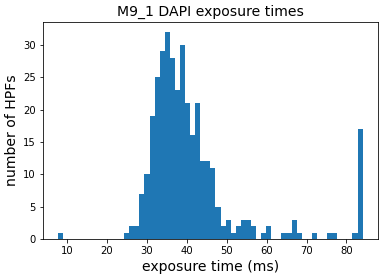
\includegraphics[width=0.32\textwidth]{images/introduction/exposure_times_M9_1_layer_1}
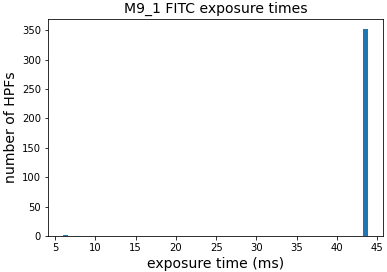
\includegraphics[width=0.32\textwidth]{images/introduction/exposure_times_M9_1_layer_10}
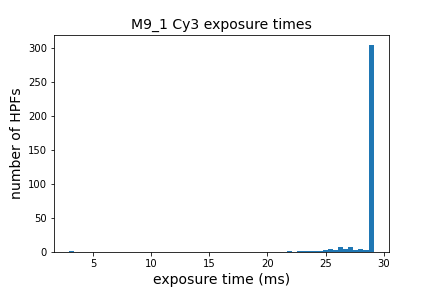
\includegraphics[width=0.32\textwidth]{images/introduction/exposure_times_M9_1_layer_19}
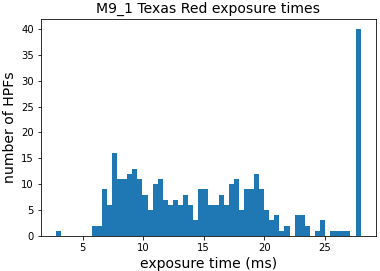
\includegraphics[width=0.32\textwidth]{images/introduction/exposure_times_M9_1_layer_26}
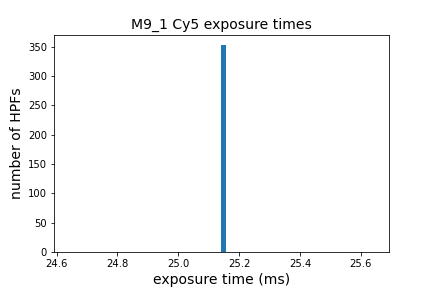
\includegraphics[width=0.32\textwidth]{images/introduction/exposure_times_M9_1_layer_33}
\caption{\footnotesize Exposure times for different layers of HPFs in the dataset \texttt{M9\_1}. Shown from top left to bottom right are layers 1, 10, 19, 26, and 33, respectively, corresponding to the first layers in each of the DAPI, FITC, Cy3, Texas Red, and Cy5 filter groups, respectively. The DAPI and Texas Red layers show substantial variation in exposure time, while the FITC and Cy3 layers show less variation for this sample, and the Cy5 layers of every HPF were all recorded with the same exposure time.}
\label{fig:exposure_time_variation_M9_1}
\end{figure}

Two example image layers with the minimum and maximum exposure times in the FITC filter group for this sample are shown in \reffig{fig:max_min_M9_1_fitc_images} to illustrate the behavior of the saturation protection feature. The minimally-exposed image layer clearly shows the single bright spot that triggered the saturation protection, stopping exposure of that HPF layer before it could be completely washed out by the noise from the spot. The maximally-exposed image layer shows no such localized brightness, and so it was exposed for the full, maximum time specified in the protocol.

\begin{figure}[!ht]
\centering
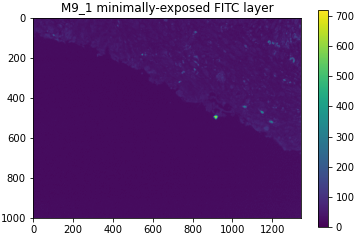
\includegraphics[width=0.49\textwidth]{images/introduction/min_exposure_M9_1_fitc_image}
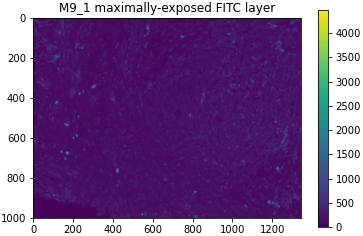
\includegraphics[width=0.49\textwidth]{images/introduction/max_exposure_M9_1_fitc_image}
\caption{\footnotesize Example images in layer 11 (corresponding to the FITC filter group) in the dataset \texttt{M9\_1} with the minimum (left) and maximum (right) recorded exposure time. The image layer with the minimum exposure time shows a clear bright spot that triggered the saturation protection feature in the Vectra 3.0 microscope software.}
\label{fig:max_min_M9_1_fitc_images}
\end{figure}

But comparing the actual numbers of counts in these image layers shows a challenge that arises from curtailing the exposure of some HPF layers. In the HPF whose FITC layers were exposed for the full, maximum time of 43.8 ms, the fluorescent tissue regions often register over a thousand counts, but the fluorescent tissue visible in the HPF layer exposed for the minimum time of 6.0 ms rarely registers more than a couple hundred counts. While a visual comparison is easily made for a human observer who can recognize that the minimally-exposed image layer shows some dark background, some tissue, and a bright spot, a quantitative comparison of the image counts themselves would not necessarily lead to the same conclusion.

Another way in which exposure time settings and the saturation protection feature can complicate analysis happens when the maximum exposure time is set too high for the typical tissue in the specimen. When the maximum exposure time is set too high, \textit{most} images saturate and are recorded with some smaller, often unique exposure time, like what is seen in the DAPI layer for the \texttt{M9\_1} sample. Two example image layers with the median and maximum exposure times in this layer group are shown in \reffig{fig:med_min_M9_1_dapi_images}. In this case, the epiethilial tissue visible in the image layer with the maximum exposure time (84.0 ms) is relatively dim, but most DAPI layers in the sample show the much brighter cells that are visible in the example image layer with the median exposure time (38.0 ms). When this even greater amount of variation is observed for a group of sample layers, the result is a large number of images whose numbers of counts do not directly translate to the brightness of the fluorescent tissue at each location within the sample.

\begin{figure}[!ht]
\centering
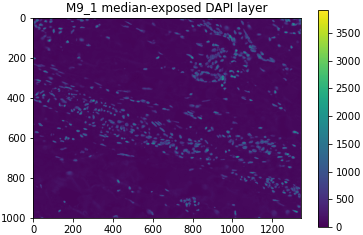
\includegraphics[width=0.49\textwidth]{images/introduction/med_exposure_M9_1_dapi_image}
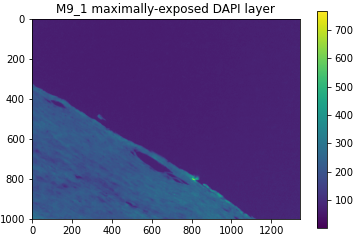
\includegraphics[width=0.49\textwidth]{images/introduction/max_exposure_M9_1_dapi_image}
\caption{\footnotesize Example images in layer 1 (corresponding to the DAPI filter group) in the dataset \texttt{M9\_1} with the median (left) and maximum (right) recorded exposure times. The image layer with the median exposure time shows typically-illuminated cells that were interpreted as bright spots by the saturation protection feature after the maximum exposure time was set using the relatively much dimmer epithelial tissue visible in the image layer with the maximum exposure time.}
\label{fig:med_min_M9_1_dapi_images}
\end{figure}

Differences in exposure time can be simply compensated for by considering counts per unit time rather than total counts, and the inForm and Phenochart softwares both offer ``normalized for exposure'' analysis modes that do exactly that \cite{inform_user_manual,phenochart_user_manual}. While this simple correction may be effective for qualitative or visual analysis of images, it is not sufficient for highly automated and quantitative analyses that rely on image data being as accurate and consistent as possible across large numbers of independent samples. 

The more sophisticated model discussed in this note applies corrections that are still linear, in that the number of counts collected increases proportionally to the total exposure time, but with an important offset for a small number of counts, called the ``dark current,'' representing noise in the camera that is present regardless of exposure to fluorescent tissue. This small, time-independent dark current is determined almost entirely by the gain, readout noise, and DC offset of the camera used to collect the microscopy images \cite{doi:10.1111/j.1365-2818.2011.03581.x}, and including it in the linear correction model is especially important for dim images whose true signal content may be comparable to the small noise in the first place.

The structure of this note is as follows. \refsec{sec:methods} describes the methods developed and the data used to measure the dark current offset as a function of image layer using portions of tissue that are multiply imaged in an overlapping fashion. \refsec{sec:results} details the results of the investigations, and the impact that applying the correction model has compared to the simpler type of correction made in the inForm and Phenochart softwares. \refsec{sec:summary} gives a brief summary. At the end of the note, Appendix~\ref{sec:impact_on_background_threshold} provides a qualitative discussion of the impact the corrections have in finding background thresholds for masking tissue regions out of images.

%%%%%%%%%%%%%%%%%%%%%%%%%%%%%%%%%%%%%%%%%%%%%% METHODS SECTION %%%%%%%%%%%%%%%%%%%%%%%%%%%%%%%%%%%%%%%%%%%%%%
\section{Methods}
\label{sec:methods}

The number of counts attributable to the dark current noise is measured as a function of image layer for several samples independently. Each measurement is made using a large set of HPF regions that each correspond to a portion of the whole slide that has been imaged more than once with different exposure times. These HPF regions are modified to account for known differences in their contents and corrected to identical exposure times, and the dark current offset is found by minimizing the pixel-averaged difference between them. Several independent measurements in each set of layers corresponding to a broadband filter group are combined to find the overall best correction factors to use. 

\subsection{General procedure}
\label{ssec:general_procedure}

When a slide is automatically scanned using the Vectra 3.0 or Vectra Polaris systems, an initial overview image is first collected at low magnification to determine where the tissue of interest is located within the slide. The microscope software then defines a rectangular grid overlaid on that tissue region, where each rectangle is a single HPF that must be collected so that the entire tissue region can be imaged at high magnification. The grid of HPFs is arranged with 20\% overlap between adjacent fields, meaning that some portions of the slide are imaged multiple times. These multiply-imaged ``overlap'' regions are used in a number of analyses to improve the quality of the overall composite high-magnification image, including registering individual HPF locations into a global coordinate system with sub-pixel accuracy, as discussed in~\cite{Heshy}.

Sometimes, two overlapping HPFs are recorded with different exposure times. When this happens, both image regions show identical content (within some caveats discussed below) at different scales of illumination. One such example of an overlap where the individual HPF image layers were recorded with difference exposure times is shown in \reffig{fig:raw_M9_1_overlap_66}, for the 66th overlap in the \texttt{M9\_1} sample. The comparison shows that the two image regions have similar content in substance, but at slightly different scales of illumination due to the differences in exposure times. 

\begin{figure}[!ht]
\centering
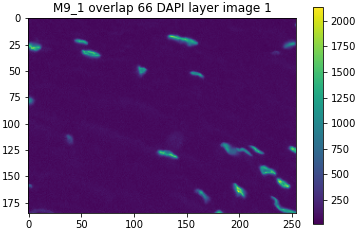
\includegraphics[width=0.49\textwidth]{images/methods/raw_M9_1_overlap_66_dapi_image_1}
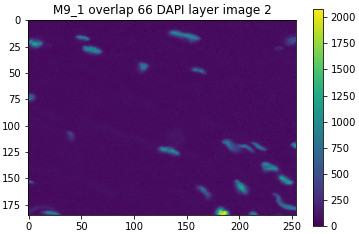
\includegraphics[width=0.49\textwidth]{images/methods/raw_M9_1_overlap_66_dapi_image_2}
\caption{\footnotesize First layer of the 66th overlap region in the \texttt{M9\_1} sample. The left image shows the lower left corner of an HPF whose first layer was exposed for 35.0 ms, and the right image shows the upper right hand corner of an adjacent HPF whose first layer was exposed for 30.0 ms.}
\label{fig:raw_M9_1_overlap_66}
\end{figure}

If the total number of counts recorded at a given pixel is modeled as some constant number of dark current counts, plus some number of counts from the fluorescent tissue that increases proportional to the amount of time the tissue is exposed to the camera, the dark current can be determined by minimizing the difference of the two HPF contents within the overlapping region.

To illustrate this concept more explicitly, consider two overlap image regions $I_{ijm}$ and $I^{\prime}_{ijm}$, represented as three-dimensional tensors whose contents are the number of counts recorded by the camera and the $i=1, \ldots, h$, $j = 1, \ldots, w$, and $m = 1, \ldots, L$ indices range over the height ($h$ pixels), width ($w$ pixels), and number of image layers $L$, respectively, of the overlap in question. If the two HPFs of which $I$ and $I^{\prime}$ are subsets are recorded with layer-dependent exposure times $t_{m}$ and $t^{\prime}_{m}$, respectively, then the number of counts at each pixel can be modelled linearly as
\begin{equation}
I_{ijm} = D_{m} + F_{ijm} t_{m} \hspace{0.08\textwidth} \mathrm{and} \hspace{0.08\textwidth} I^{\prime}_{ijm} = D_{m} + F_{ijm} t^{\prime}_{m},
\end{equation}
where $D_{m}$ is the constant number of counts from the dark current in the given image layer, and $F_{ijm}$ represents the luminous flux (in counts per unit time) of the underlying fluorescent tissue incident on each pixel. Note that while the dark current should, theoretically, be the same in each image layer, the actual noise may vary over time as the multiply-stained samples are successively illuminated at different wavelengths of light, and so we measure the number of dark current counts independently in each image layer.

Because the true $F_{ijm}$ are unknown, the numbers of dark current counts must be estimated a-posteriori. To that end, for arbitrary dark current offsets $D_{m}$, we define $\Iota_{ijm}$ and $\Iota^{\prime}_{ijm}$, the overlapping image regions corrected to the same sample-median exposure times $t_{m}^{\mathrm{med}}$, as
\begin{equation}
\Iota_{ijm} = 
\begin{cases} 
      D_{m}+\left(\frac{t_{m}^{\mathrm{med}}}{t_{m}}\right)\left(I_{ijm}-D_{m}\right) & I_{ijm} > D_{m}  \\
      I_{ijm} & I_{ijm} \leq D_{m} 
\end{cases}
\label{eq:image_corr_def_1}
\end{equation}
and
\begin{equation}
\Iota^{\prime}_{ijm} = 
\begin{cases} 
      D_{m}+\left(\frac{t_{m}^{\mathrm{med}}}{t^{\prime}_{m}}\right)\left(I^{\prime}_{ijm}-D_{m}\right) & I^{\prime}_{ijm} > D_{m}  \\
      I^{\prime}_{ijm} & I^{\prime}_{ijm} \leq D_{m} 
\end{cases}
.
\label{eq:image_corr_def_2}
\end{equation}

With this correction procedure defined, the best estimate of the dark current in each layer can then be determined by minimizing the L1-norm cost representing the difference in corrected overlap region image contents observed in a sufficiently large set of overlaps with different exposure times, averaged over the total number of pixels, like
\begin{equation}
D = \argmin{ \left[ \frac{ \sum_{n=1}^{N} \left( \sum_{i=1}^{h_{n}} \sum_{j=1}^{w_{n}} \left| \Iota_{n} - \Iota^{\prime}_{n} \right| \right) }{ \sum_{n=1}^{N} h_{n}w_{n}} \right] },
\label{eq:minimization_def}
\end{equation} 
where the $m$ index has been suppressed because the results are independent in each image layer, and the subscript $n=1,\ldots,N$ is used to distinguish each of $N$ total overlap regions with independent heights $h_{n}$ and widths $w_{n}$. 

This minimization procedure is performed individually for each scanned slide, identically for every image layer, using every overlapping HPF pair where the two images were recorded with different exposure times. The overall optimal values of $D_{m}$ are the average of the results for each slide, weighted by the total number of pixels used in each layer's fit.  

\subsection{Data used}
\label{ssec:data_used}

The HPF image regions used to determine the numbers of dark current counts come from 19 slides scanned using the Vectra 3.0 and 26 slides scanned using the Vectra Polaris. Not every slide contributes to the measurements in every layer, because the distributions of HPF exposure times are unique for every sample and for every group of layers imaged using the same broadband filter cube. 

The slides used in each layer group are those that have at least 1500 overlaps with differing HPF exposure times, after neglecting any overlaps where at least one HPF is located on the edge of the slide's tissue region (to minimize the amount of empty background included), and only counting overlaps that are bright and distinct enough to be pairwise-aligned using the procedure detailed in \cite{Heshy}. Up to ten slides are used in each layer group, sorted by the number of overlaps they contribute. \reffig{fig:n_overlaps_used_vectra} shows the numbers of overlaps used to independently estimate the dark current for each sample in each layer for the slides collected using the Vectra 3.0 microscope, and \reffig{fig:n_overlaps_used_polaris} shows the same for the slides collected with the Vectra Polaris microscope. Layers 10 and 11 in the Vectra Polaris slides were all recorded with identical exposure times, and so no estimates of the dark current offsets can (or must) be made for those layers. 

\begin{figure}[!ht]
\centering
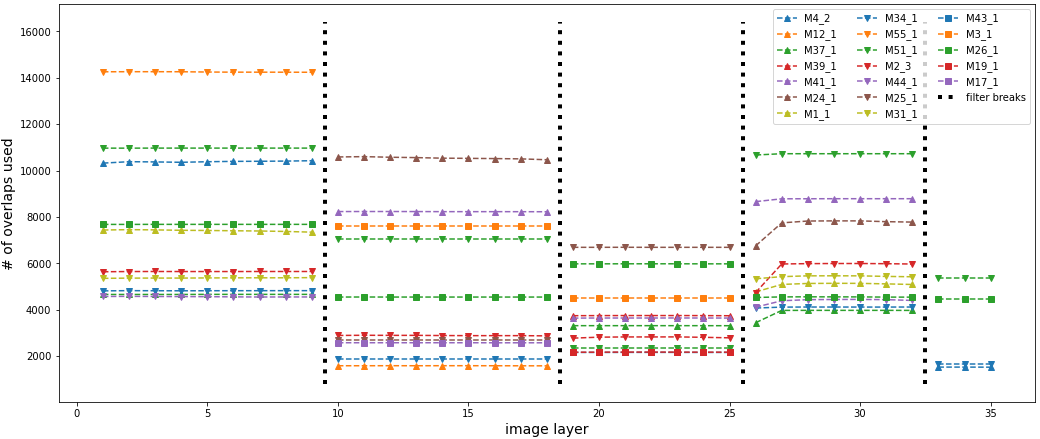
\includegraphics[width=0.98\textwidth]{images/methods/n_overlaps_used_vectra}
\caption{\footnotesize Number of overlaps used from each sample to determine the dark current in each image layer for images collected with the Vectra 3.0 microscope. The thick dotted black lines separate layers imaged with different filter cubes.}
\label{fig:n_overlaps_used_vectra}
\end{figure}

\begin{figure}[!ht]
\centering
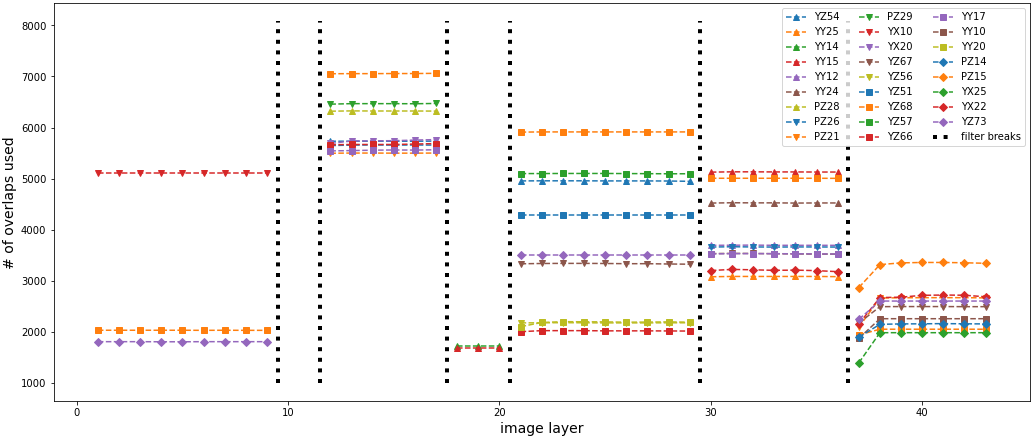
\includegraphics[width=0.98\textwidth]{images/methods/n_overlaps_used_polaris}
\caption{\footnotesize Number of overlaps used from each sample to determine the dark current in each image layer for images collected with the Vectra Polaris microscope. The thick dotted black lines separate layers imaged with different filter cubes. Layers 10 and 11 of every image have the same exposure time, so no estimate of the dark current is made for those layers. }
\label{fig:n_overlaps_used_polaris}
\end{figure}

\subsection{Corrections to raw data}
\label{ssec:corrections_to_raw_data}

The raw image region data are not expected to depict exactly the same content even if they are recorded with identical exposure times due to a number of known effects, and so the images are pre-processed to bring them as near to agreement (except for exposure time differences) as possible. The images used are first gently smoothed using a 3 pixel-wide Gaussian filter to remove small-scale random noise. \reffig{fig:smoothed_M9_1_overlap_66} shows the same two overlapping image layer regions as \reffig{fig:raw_M9_1_overlap_66} after this smoothing is performed.

\begin{figure}[!ht]
\centering
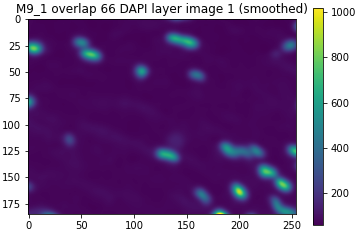
\includegraphics[width=0.49\textwidth]{images/methods/smoothed_M9_1_overlap_66_dapi_image_1}
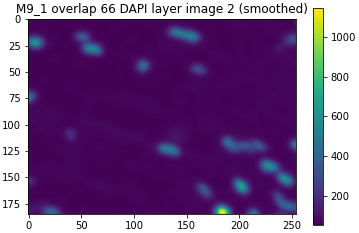
\includegraphics[width=0.49\textwidth]{images/methods/smoothed_M9_1_overlap_66_dapi_image_2}
\caption{\footnotesize First layer of the 66th overlap region in the \texttt{M9\_1} sample, after smoothing by a 3 pixel-wide Gaussian filter. The image layer on the left was exposed for 35.0 ms, and the image layer on the right was exposed for 30.0 ms.}
\label{fig:smoothed_M9_1_overlap_66}
\end{figure}

Another known difference between the two overlapping image regions is systematic and spatially-dependent variation in the illumination of each HPF. This effect, called ``flatfielding,'' is particularly important because the overlapping regions come from different portions of the two HPFs: for example, the left-hand side of one image overlaps with the right-hand side of another, and the two sides of the images are overall illuminated differently. Flatfielding, and the method for deriving correction factors for it, are discussed in \cite{flatfielding_note}, and the relevant corrections for each microscope are applied to each HPF. The only difference between the applied corrections and those derived using the full procedure in \cite{flatfielding_note} is that the masking procedure is skipped, as corrections for differences in exposure time are integral to estimation of the background thresholds (see Appendix~\ref{sec:impact_on_background_threshold}) and therefore the determinations of the tissue region masks. 

\reffig{fig:applied_flatfield_layers_vectra} shows examples of the flatfielding corrections applied to HPFs imaged with the Vectra 3.0 microscope for the first, middle, and last layers in each broadband filter region. Figures~\ref{fig:applied_flatfield_layers_polaris_1} and \ref{fig:applied_flatfield_layers_polaris_2} show the same, except for the corrections applied to HPFs imaged with the Vectra Polaris microscope. \reffig{fig:smoothed_flatfielded_M9_1_overlap_66} shows the same example overlapping image regions as in \reffig{fig:smoothed_M9_1_overlap_66} after application of the flatfield corrections.

\begin{figure}[!ht]
\centering
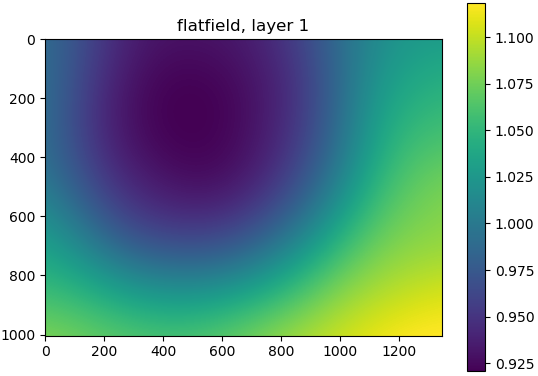
\includegraphics[width=0.32\textwidth]{images/methods/flatfield_layers_vectra/flatfield_layer_1}
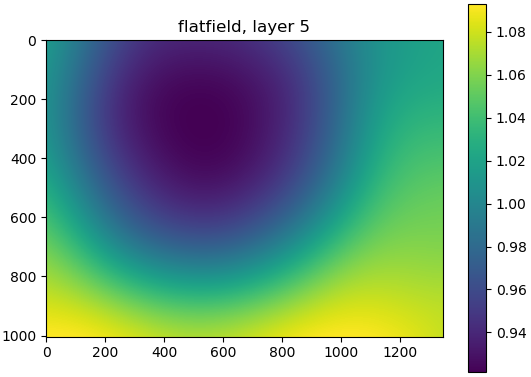
\includegraphics[width=0.32\textwidth]{images/methods/flatfield_layers_vectra/flatfield_layer_5}
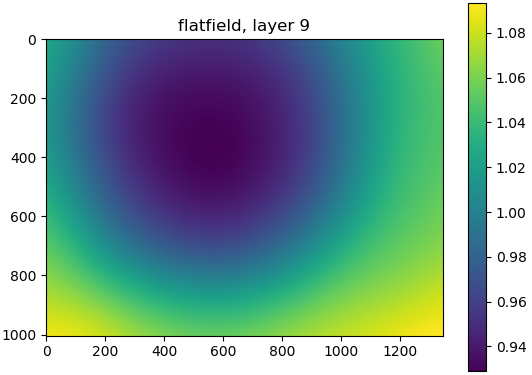
\includegraphics[width=0.32\textwidth]{images/methods/flatfield_layers_vectra/flatfield_layer_9}
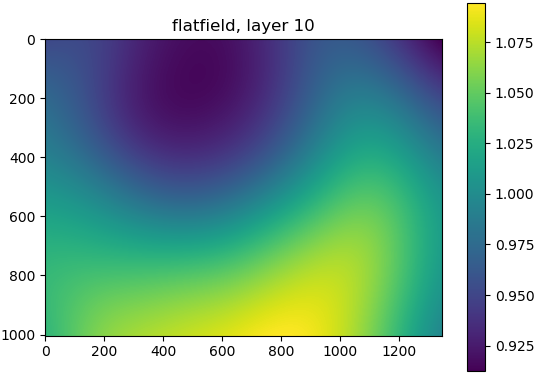
\includegraphics[width=0.32\textwidth]{images/methods/flatfield_layers_vectra/flatfield_layer_10}
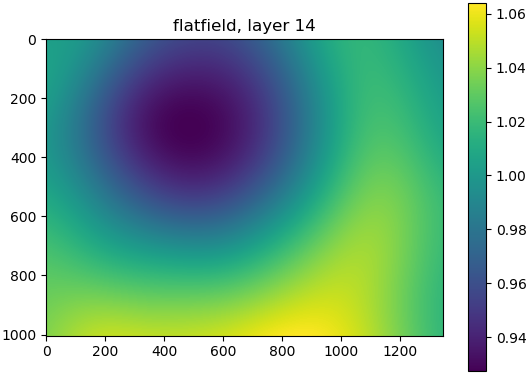
\includegraphics[width=0.32\textwidth]{images/methods/flatfield_layers_vectra/flatfield_layer_14}
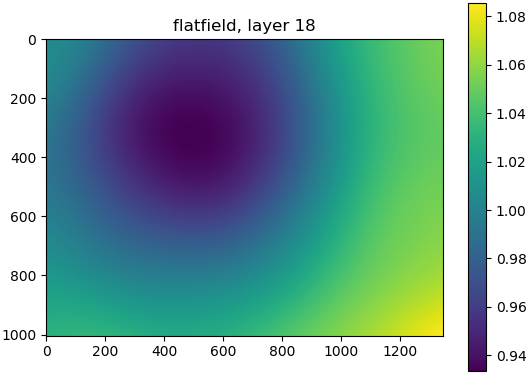
\includegraphics[width=0.32\textwidth]{images/methods/flatfield_layers_vectra/flatfield_layer_18}
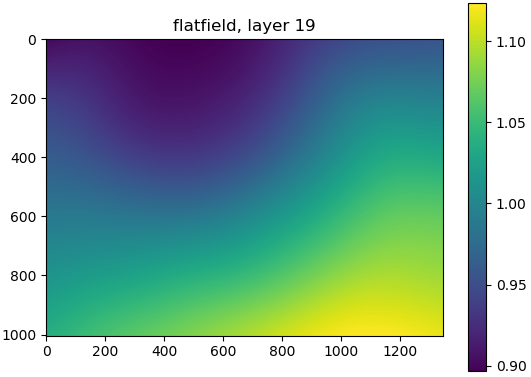
\includegraphics[width=0.32\textwidth]{images/methods/flatfield_layers_vectra/flatfield_layer_19}
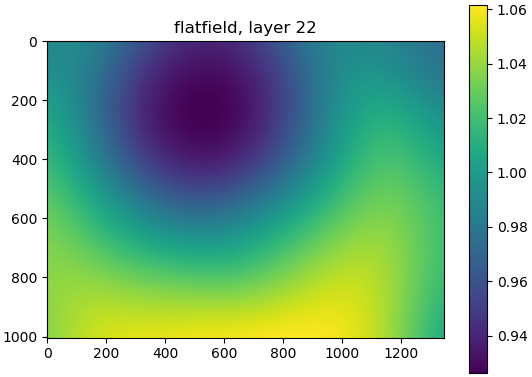
\includegraphics[width=0.32\textwidth]{images/methods/flatfield_layers_vectra/flatfield_layer_22}
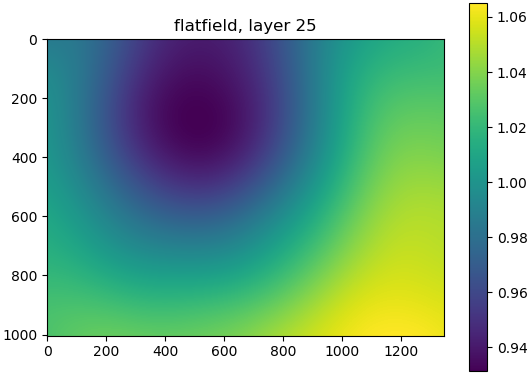
\includegraphics[width=0.32\textwidth]{images/methods/flatfield_layers_vectra/flatfield_layer_25}
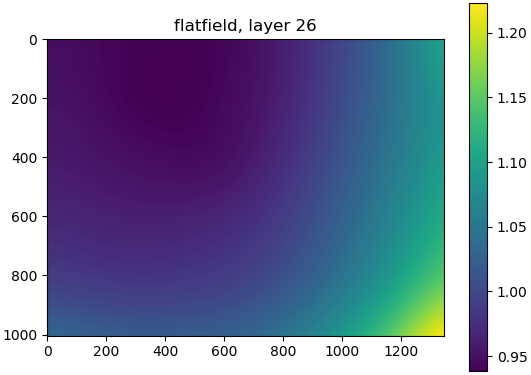
\includegraphics[width=0.32\textwidth]{images/methods/flatfield_layers_vectra/flatfield_layer_26}
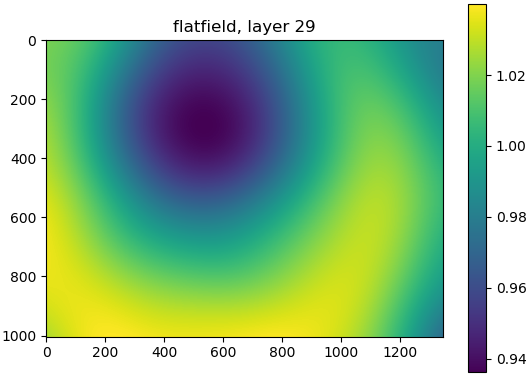
\includegraphics[width=0.32\textwidth]{images/methods/flatfield_layers_vectra/flatfield_layer_29}
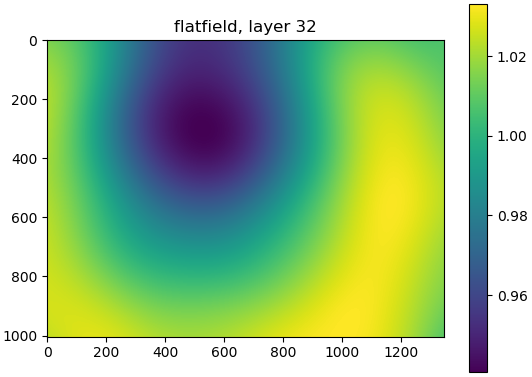
\includegraphics[width=0.32\textwidth]{images/methods/flatfield_layers_vectra/flatfield_layer_32}
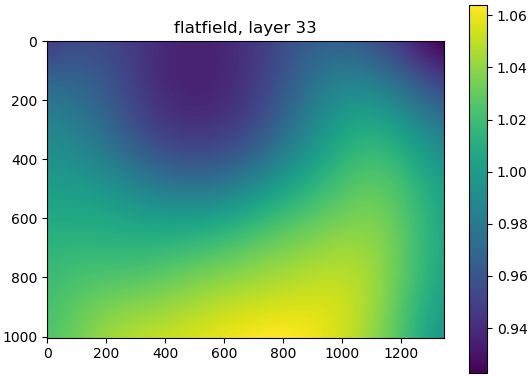
\includegraphics[width=0.32\textwidth]{images/methods/flatfield_layers_vectra/flatfield_layer_33}
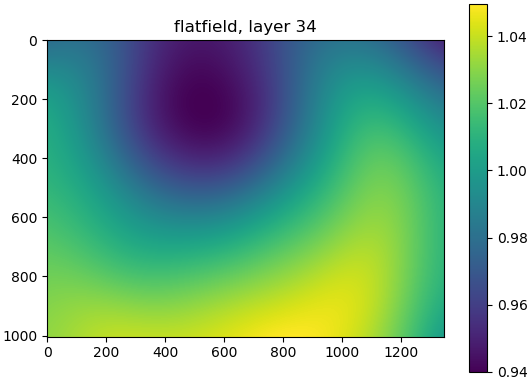
\includegraphics[width=0.32\textwidth]{images/methods/flatfield_layers_vectra/flatfield_layer_34}
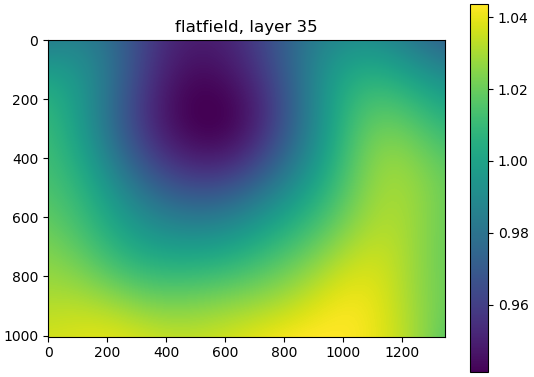
\includegraphics[width=0.32\textwidth]{images/methods/flatfield_layers_vectra/flatfield_layer_35}
\caption{\footnotesize Flatfield correction factors applied to HPFs imaged with the Vectra 3.0 microscope in layers 1, 5, 9, 10, 14, 18, 29, 22, 25, 26, 29, 32, 33, 34, and 35, from upper left to lower right, respectively.}
\label{fig:applied_flatfield_layers_vectra}
\end{figure}

\begin{figure}[!ht]
\centering
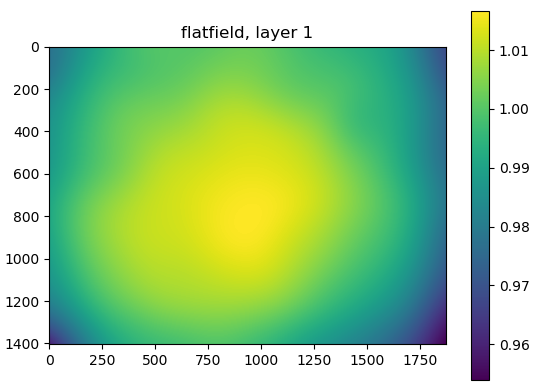
\includegraphics[width=0.32\textwidth]{images/methods/flatfield_layers_polaris/flatfield_layer_1}
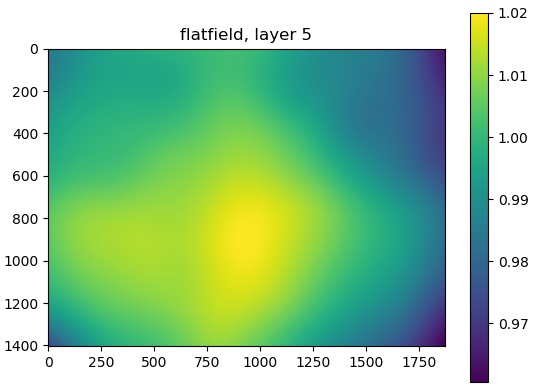
\includegraphics[width=0.32\textwidth]{images/methods/flatfield_layers_polaris/flatfield_layer_5}
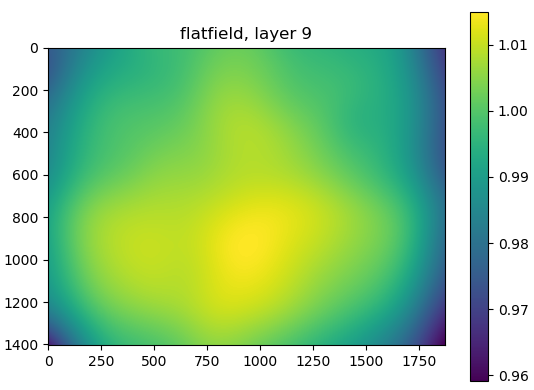
\includegraphics[width=0.32\textwidth]{images/methods/flatfield_layers_polaris/flatfield_layer_9}
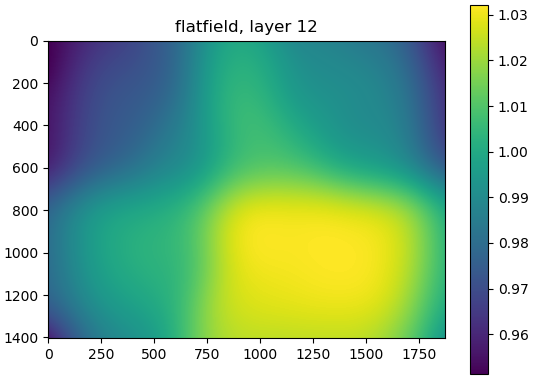
\includegraphics[width=0.32\textwidth]{images/methods/flatfield_layers_polaris/flatfield_layer_12}
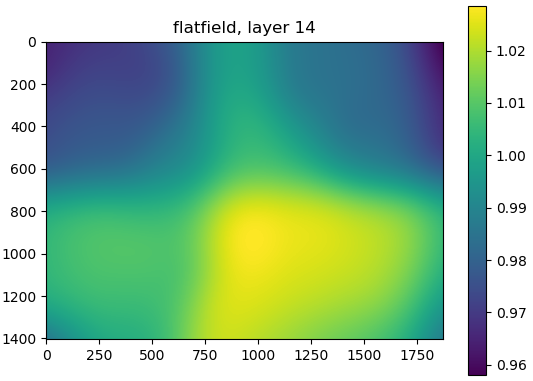
\includegraphics[width=0.32\textwidth]{images/methods/flatfield_layers_polaris/flatfield_layer_14}
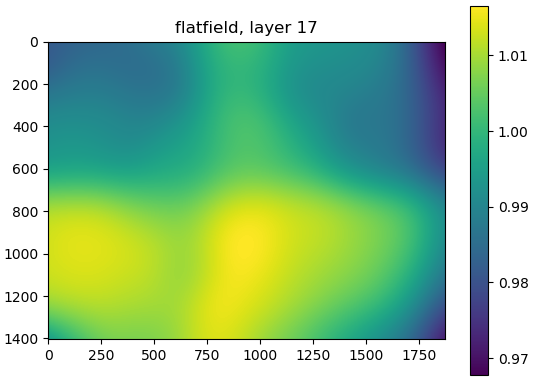
\includegraphics[width=0.32\textwidth]{images/methods/flatfield_layers_polaris/flatfield_layer_17}
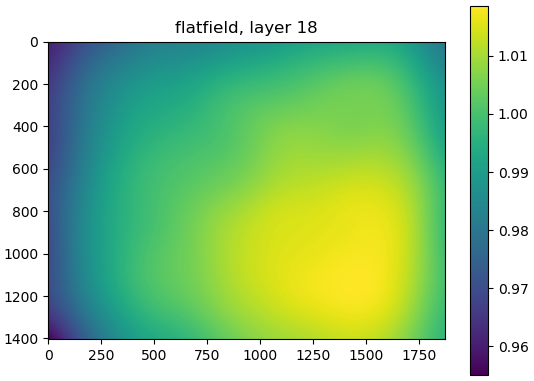
\includegraphics[width=0.32\textwidth]{images/methods/flatfield_layers_polaris/flatfield_layer_18}
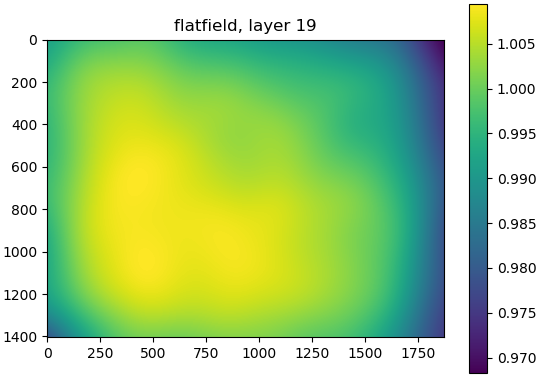
\includegraphics[width=0.32\textwidth]{images/methods/flatfield_layers_polaris/flatfield_layer_19}
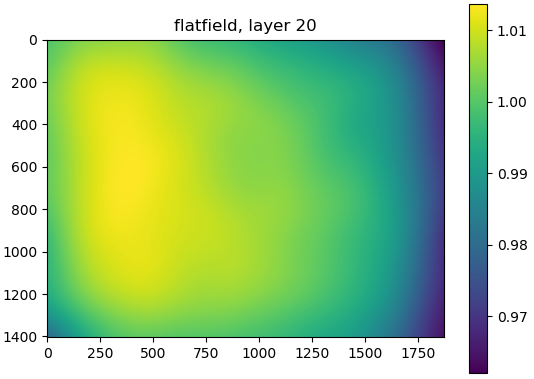
\includegraphics[width=0.32\textwidth]{images/methods/flatfield_layers_polaris/flatfield_layer_20}
\caption{\footnotesize Flatfield correction factors applied to HPFs imaged with the Vectra Polaris microscope in layers 1, 5, 9, 12, 14, 17, 18, 19, and 20, from upper left to lower right, respectively.}
\label{fig:applied_flatfield_layers_polaris_1}
\end{figure}

\begin{figure}[!ht]
\centering
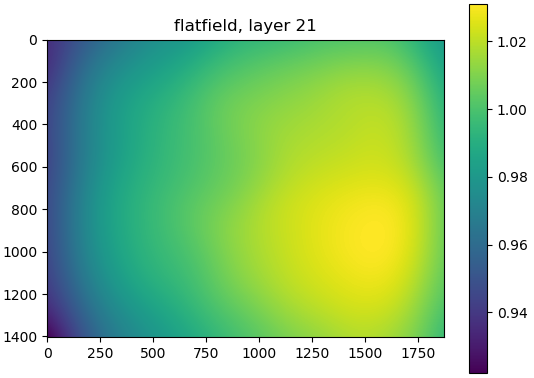
\includegraphics[width=0.32\textwidth]{images/methods/flatfield_layers_polaris/flatfield_layer_21}
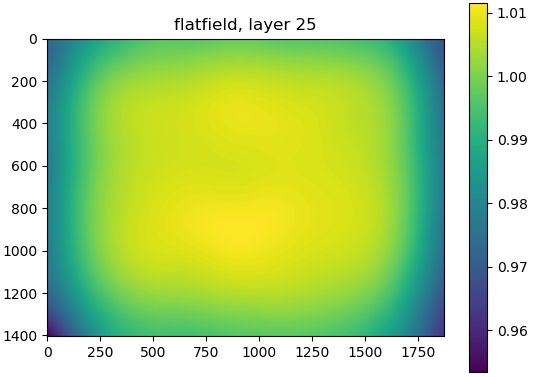
\includegraphics[width=0.32\textwidth]{images/methods/flatfield_layers_polaris/flatfield_layer_25}
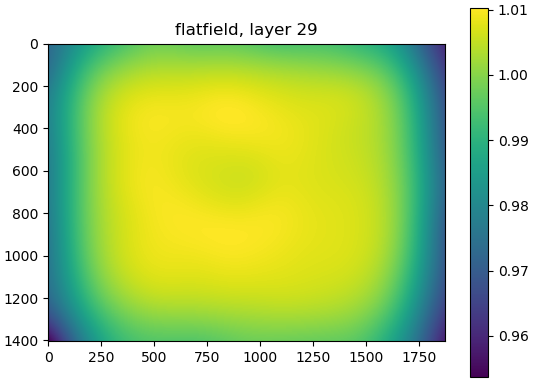
\includegraphics[width=0.32\textwidth]{images/methods/flatfield_layers_polaris/flatfield_layer_29}
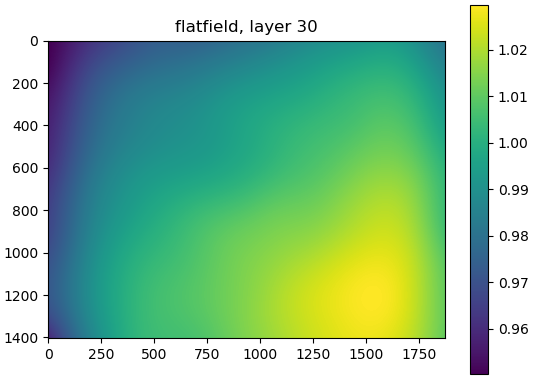
\includegraphics[width=0.32\textwidth]{images/methods/flatfield_layers_polaris/flatfield_layer_30}
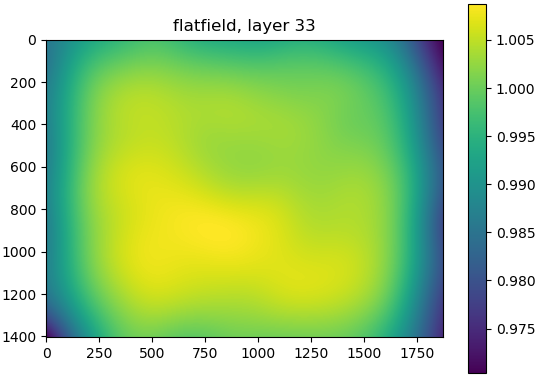
\includegraphics[width=0.32\textwidth]{images/methods/flatfield_layers_polaris/flatfield_layer_33}
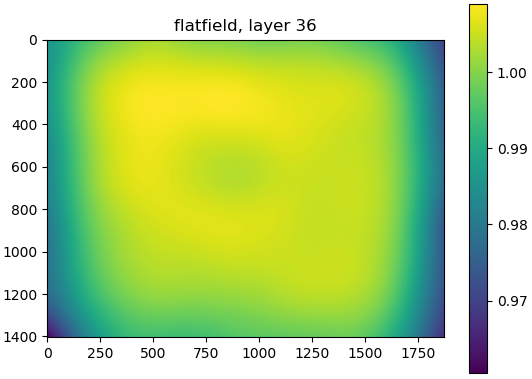
\includegraphics[width=0.32\textwidth]{images/methods/flatfield_layers_polaris/flatfield_layer_36}
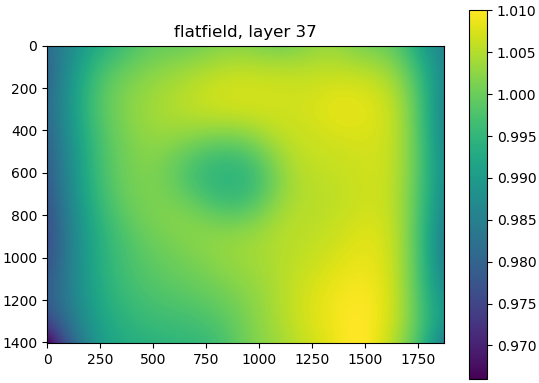
\includegraphics[width=0.32\textwidth]{images/methods/flatfield_layers_polaris/flatfield_layer_37}
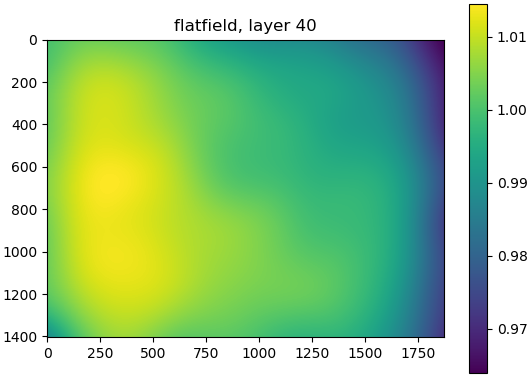
\includegraphics[width=0.32\textwidth]{images/methods/flatfield_layers_polaris/flatfield_layer_40}
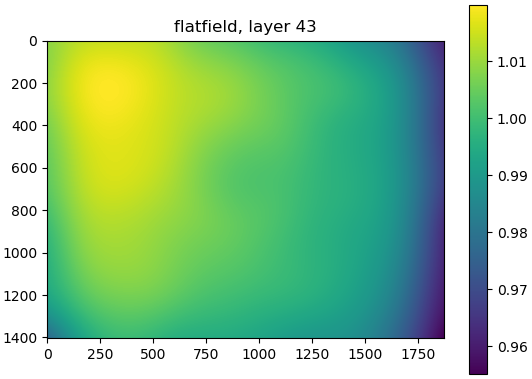
\includegraphics[width=0.32\textwidth]{images/methods/flatfield_layers_polaris/flatfield_layer_43}
\caption{\footnotesize Flatfield correction factors applied to HPFs imaged with the Vectra Polaris microscope in layers 21, 25, 29, 30, 33, 36, 37, 40, and 43, from upper left to lower right, respectively.}
\label{fig:applied_flatfield_layers_polaris_2}
\end{figure}

\begin{figure}[!ht]
\centering
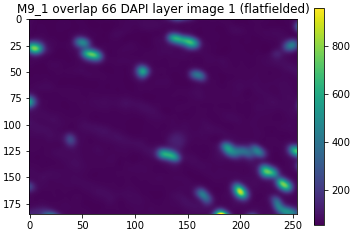
\includegraphics[width=0.49\textwidth]{images/methods/smoothed_flatfielded_M9_1_overlap_66_dapi_image_1}
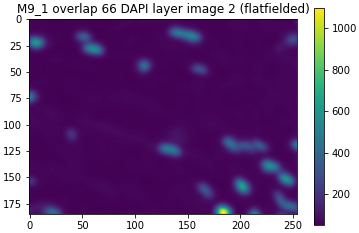
\includegraphics[width=0.49\textwidth]{images/methods/smoothed_flatfielded_M9_1_overlap_66_dapi_image_2}
\caption{\footnotesize First layer of the 66th overlap region in the \texttt{M9\_1} sample, after smoothing by a 3 pixel-wide Gaussian filter and application of flatfield correction factors. The image layer on the left was exposed for 35.0 ms, and the image layer on the right was exposed for 30.0 ms.}
\label{fig:smoothed_flatfielded_M9_1_overlap_66}
\end{figure}

Next, while the spatial extents of the overlapping regions (i.e. the exact subsets of the total images to use) are technically defined by the 20\% boundaries around each HPF, there are often minute relative translations of the microscope stage that occur between imaging of individual HPFs that makes these boundaries imperfect at the scale of a few pixels. The registrations of these image regions to a shared local coordinate system must therefore be performed using the pair-wise alignment procedure discussed in \cite{Heshy} to ensure the image regions in each overlap aren't translated relative to one another. 

\reffig{fig:smoothed_flatfielded_aligned_M9_1_overlap_66} shows the same image regions as in \reffig{fig:smoothed_flatfielded_M9_1_overlap_66} after they have been pairwise aligned. In addition to showing the two image layer regions separately, \reffig{fig:smoothed_flatfielded_aligned_M9_1_overlap_66} also shows them overlaid on one another in a false color image, where the HPF on the left hand side is colored magenta and the other is colored green, so that the resulting overlay appears white when the two image contents are identical and more magenta or green when one image is brighter than the other. In this example, the false color overlay appears magenta overall in color because the left-hand image was exposed for longer.

\begin{figure}[!ht]
\centering
\includegraphics[width=0.49\textwidth]{images/methods/smoothed_flatfielded_aligned_M9_1_overlap_66_dapi_image_1}
\includegraphics[width=0.49\textwidth]{images/methods/smoothed_flatfielded_aligned_M9_1_overlap_66_dapi_image_2}
\includegraphics[width=0.49\textwidth]{images/methods/smoothed_flatfielded_aligned_M9_1_overlap_66_dapi_overlay}
\caption{\footnotesize Upper: first layer of the 66th overlap region in the \texttt{M9\_1} sample, after smoothing by a 3 pixel-wide Gaussian filter, application of flatfield correction factors, and small relative translations determined by pairwise alignment. The image layer on the left was exposed for 35.0 ms, and the image layer on the right was exposed for 30.0 ms. Lower: false color overlay of the two images in the upper part of the figure, where the left-hand image is colored magenta and the right hand image is colored green.}
\label{fig:smoothed_flatfielded_aligned_M9_1_overlap_66}
\end{figure}

Finally, a last known difference between the overlap images is spatially-dependent ``warping'' effects introduced by the microscope camera. The exact warping patterns can only be measured following precise corrections for exposure time differences and flatfielding, but it is known that the effects are generally largest on the edges of each HPF. Therefore, the spatial extent of each overlapping region in the local coordinate system is restricted to the central 50\% in each of the height and width dimensions, and only about 25\% of the total overlapping area is used in each pair of images. This central image portion also corresponds to the extent of the central 64\%, or ``primary region'', of each HPF that is ultimately used for pathology analysis. \reffig{fig:smoothed_flatfielded_aligned_clipped_M9_1_overlap_66} shows the final images used to calculate the cost from the 66th overlap in \texttt{M9\_1}, after all corrections are applied and the outer 75\% of each image is cut out, as well as the false color overlay of the two images. The predominant remaining difference in the images (as is visible in the false color overlay) is the overall scale of illumination due to the differences in exposure times. 

\begin{figure}[!ht]
\centering
\includegraphics[width=0.49\textwidth]{images/methods/smoothed_flatfielded_aligned_clipped_M9_1_overlap_66_dapi_image_1}
\includegraphics[width=0.49\textwidth]{images/methods/smoothed_flatfielded_aligned_clipped_M9_1_overlap_66_dapi_image_2}
\includegraphics[width=0.49\textwidth]{images/methods/smoothed_flatfielded_aligned_clipped_M9_1_overlap_66_dapi_overlay}
\caption{\footnotesize Upper: first layer of the 66th overlap region in the \texttt{M9\_1} sample, after smoothing by a 3 pixel-wide Gaussian filter, application of flatfield correction factors and alignment shifts, and removal of the outer (lower left) 75\% portions of each image. The image layer on the left was exposed for 35.0 ms, and the image layer on the right was exposed for 30.0 ms. Lower: false color overlay of the two images in the upper part of the figure, where the left-hand image is colored magenta and the right hand image is colored green.}
\label{fig:smoothed_flatfielded_aligned_clipped_M9_1_overlap_66}
\end{figure}

\clearpage

\subsection{Performing minimization}
\label{ssec:performing_minimization}

Theoretically, there should not be any pixels in any image observed with a number of counts less than the constant noise from the dark current, but this is not the case in practice due to random noise and Poisson count error. This possible undercounting is the reason for the cases with $I_{ijm} \leq D_{m}$ and $I^{\prime}_{ijm} \leq D_{m}$ in \refeq{eq:image_corr_def_1} and \refeq{eq:image_corr_def_2}, but these cases may also bias the minimization results toward larger values of $D_{m}$. To prevent any bias, then, an upper bound is set on the allowed values of $D_{m}$ for the minimization in each sample and layer. This upper bound is set at the smallest integer value for which more than 0.01\% of the pixels in any image have counts less than the upper bound.

Calculating the cost of any individual overlap as defined in \refeq{eq:minimization_def} requires comparing every pair of individual pixel values, which consumes a significant amount of computational memory when a large number of overlaps is used in the minimization. To reduce the amount of memory required, the cost from each individual overlap is calculated from a pre-determined curve, instead of from the image pixel contents, during minimization. Each overlap's true cost is calculated as the images are first read in at 100 evenly-spaced values between zero and the upper bound on $D$, and then during minimization the cost is calculated by linearly interpolating between the nearest points on that predetermined curve. 

Figures ~\ref{fig:overlap_cost_examples_vectra_1}-\ref{fig:overlap_cost_examples_polaris_2} show some examples of individual overlap false color overlay comparisons before and after correction with the optimal $D$ found for their particular sample layer, along with their associated costs between the fitting bounds as calculated from the unsmoothed/flatfielded whole images and from the smoothed/flatfielded aligned central region-only images. Figures~\ref{fig:overlap_cost_examples_vectra_1} and \ref{fig:overlap_cost_examples_vectra_2} show some examples for samples imaged with the Vectra 3.0 microscope, and Figures~\ref{fig:overlap_cost_examples_polaris_1} and \ref{fig:overlap_cost_examples_polaris_2} show examples for samples imaged with the Vectra Polaris microscope. 

In every figure, the overlays in the left and center columns show the full overlap regions without smoothing, but the costs above them are calculated with the smoothed central regions of the overlaps. Both the whole/unsmoothed and central/smoothed images are corrected for flatfielding and pairwise-aligned. In the right column of each figure, costs calculated using the entire unsmoothed image regions are shown in blue, and costs calculated from the smoothed central image regions are shown in orange, while the vertical black line shows the best-fit value of $D$. The differences in image exposure times are in milliseconds. The overlays give a qualitative idea of how applying corrections for differences in exposure time brings the images closer to a mutual overall scale of illumination corresponding to the median exposure time in each sample and layer.

\begin{figure}[!ht]
\centering
\includegraphics[width=0.98\textwidth]{images/methods/cost_examples_vectra/overlay_comp_random_6761_offset=18.961}
\includegraphics[width=0.98\textwidth]{images/methods/cost_examples_vectra/overlay_comp_random_2425_offset=20.326}
\includegraphics[width=0.98\textwidth]{images/methods/cost_examples_vectra/overlay_comp_random_3946_offset=20.222}
\caption{\footnotesize Left and center columns: false color overlay comparisons before (left column) and after (center column) correction for differences in exposure times with the optimal $D$ for several sample layers imaged using the Vectra 3.0 microscope. Right column: L1-norm costs for the same overlaps at 100 values of $D$ between zero and the sample/layer-dependent upper bound. From the upper to lower rows, the overlaps shown are examples from layer 1 of \texttt{M26\_1}, layer 10 of \texttt{M17\_1}, and layer 23 of \texttt{M3\_1}, respectively.}
\label{fig:overlap_cost_examples_vectra_1}
\end{figure}

\begin{figure}[!ht]
\centering
\includegraphics[width=0.98\textwidth]{images/methods/cost_examples_vectra/overlay_comp_random_10478_offset=17.778}
\includegraphics[width=0.98\textwidth]{images/methods/cost_examples_vectra/overlay_comp_random_892_offset=21.314}
\caption{\footnotesize Left and center columns: false color overlay comparisons before (left column) and after (center column) correction for differences in exposure times with the optimal $D$ for several sample layers imaged using the Vectra 3.0 microscope. Right column: L1-norm costs for the same overlaps at 100 values of $D$ between zero and the sample/layer-dependent upper bound. From the upper to lower rows, the overlaps shown are examples from layer 31 of \texttt{M51\_1} and layer 33 of \texttt{M4\_2}, respectively.}
\label{fig:overlap_cost_examples_vectra_2}
\end{figure}

\begin{figure}[!ht]
\centering
\includegraphics[width=0.98\textwidth]{images/methods/cost_examples_polaris/overlay_comp_random_4357_offset=51.980}
\includegraphics[width=0.98\textwidth]{images/methods/cost_examples_polaris/overlay_comp_random_2668_offset=51.848}
\includegraphics[width=0.98\textwidth]{images/methods/cost_examples_polaris/overlay_comp_random_1554_offset=51.000}
\caption{\footnotesize Left and center columns: false color overlay comparisons before (left column) and after (center column) correction for differences in exposure times with the optimal $D$ for several sample layers imaged using the Vectra Polaris microscope. Right column: L1-norm costs for the same overlaps at 100 values of $D$ between zero and the sample/layer-dependent upper bound. From the upper to lower rows, the overlaps shown are examples from layer 4 of \texttt{YX10}, layer 16 of \texttt{PZ29}, and layer 19 of \texttt{YY15}, respectively.}
\label{fig:overlap_cost_examples_polaris_1}
\end{figure}

\begin{figure}[!ht]
\centering
\includegraphics[width=0.98\textwidth]{images/methods/cost_examples_polaris/overlay_comp_random_5023_offset=50.770}
\includegraphics[width=0.98\textwidth]{images/methods/cost_examples_polaris/overlay_comp_random_4697_offset=49.636}
\includegraphics[width=0.98\textwidth]{images/methods/cost_examples_polaris/overlay_comp_random_1916_offset=50.424}
\caption{\footnotesize Left and center columns: false color overlay comparisons before (left column) and after (center column) correction for differences in exposure times with the optimal $D$ for several sample layers imaged using the Vectra Polaris microscope. Right column: L1-norm costs for the same overlaps at 100 values of $D$ between zero and the sample/layer-dependent upper bound. From the upper to lower rows, the overlaps shown are examples from layer 24 of \texttt{YZ68}, layer 31 of \texttt{YY15}, and layer 40 of \texttt{PZ14}, respectively.}
\label{fig:overlap_cost_examples_polaris_2}
\end{figure}

\reffig{fig:cost_reduction_plots_M51_1_layer_30} shows a typical example (for the 30th layer of the Vectra 3.0 sample \texttt{M51\_1}) of how the costs from all the individual overlaps change as a result of applying corrections for exposure time differences with the best-fit $D$ found for this sample. Before correction, a clear correlation is visible between the difference in an overlap's image exposure times and its cost. This correlation is not present after correction. \reffig{fig:cost_reduction_plots_YZ68_layer_12} shows the same for the 12th layer of the Vectra Polaris sample \texttt{YZ68}.

\begin{figure}[!ht]
\centering
\includegraphics[width=0.98\textwidth]{images/methods/cost_reduction_plots_2d_M51_1_layer_30}
\caption{\footnotesize Two-dimensional histograms of pre-fit cost (upper left), post-fit cost (upper right), cost reduction (pre-fit minus post-fit cost) (lower left), and fractional cost reduction (cost reduction divided by pre-fit cost) (lower right) vs. difference in image exposure times for all overlaps used in the minimization for layer 30 of the Vectra 3.0 sample \texttt{M51\_1}.}
\label{fig:cost_reduction_plots_M51_1_layer_30}
\end{figure}

\begin{figure}[!ht]
\centering
\includegraphics[width=0.98\textwidth]{images/methods/cost_reduction_plots_2d_YZ68_layer_12}
\caption{\footnotesize Two-dimensional histograms of pre-fit cost (upper left), post-fit cost (upper right), cost reduction (pre-fit minus post-fit cost) (lower left), and fractional cost reduction (cost reduction divided by pre-fit cost) (lower right) vs. difference in image exposure times for all overlaps used in the minimization for layer 12 of the Vectra Polaris sample \texttt{YZ68}.}
\label{fig:cost_reduction_plots_YZ68_layer_12}
\end{figure}

\clearpage

%%%%%%%%%%%%%%%%%%%%%%%%%%%%%%%%%%%%%%%%%%%%%% RESULTS SECTION %%%%%%%%%%%%%%%%%%%%%%%%%%%%%%%%%%%%%%%%%%%%%%
\section{Results}
\label{sec:results}

The overall best values of the number of counts attributable to dark current noise in each sample and layer are presented for samples imaged using both the Vectra 3.0 and Vectra Polaris microscopes. The effect of applying corrections using these offsets is quantified by measuring differences in overlap pixel-average counts per unit time before and after correction, using sets of overlaps with different HPF exposure times in samples independent from those used to make the measurements. 

\subsection{Dark current offsets}
\label{ssec:dark_current_offsets}

The optimal dark current offsets found for each sample used are pictured in \reffig{fig:dark_current_offsets_vectra} for the 35 layers of the Vectra 3.0 samples, and in \reffig{fig:dark_current_offsets_polaris} for the 43 layers of the Vectra Polaris samples. The figures also show the final weighted average dark current offsets in each layer in black, and these values are also listed in \reftab{tab:best_offsets_vectra} for the Vectra 3.0 samples and in \reftab{tab:best_offsets_polaris} for the Vectra Polaris samples. The values found for the individual samples and overall are all very similar, but there is some dependence on the image layer, particularly for layers near the extremes of the broadband filter groups. Generally, the dark current offsets found for the Vectra Polaris samples are higher than those for the Vectra 3.0 samples.

\begin{figure}[!ht]
\centering
\includegraphics[width=0.98\textwidth]{images/results/dark_current_offsets_vectra}
\caption{\footnotesize Optimal dark current offsets found independently for each sample (dashed lines) and the overall weighted averages (solid black lines/points) in each layer for images collected with the Vectra 3.0 microscope. The thick dotted black lines separate layers imaged with different filter cubes.}
\label{fig:dark_current_offsets_vectra}
\end{figure}

\begin{table}[!htb]
\centering
\begin{tabular}{c c c}
Image layer $m$ & Number of overlaps & Overall best $D_{m}$ \\
\hline
1               & 75706              & 19.07 \\
2               & 75824              & 19.18 \\
3               & 75802              & 19.35 \\
4               & 75758              & 19.57 \\
5               & 75770              & 18.68 \\
6               & 75766              & 18.28 \\
7               & 75758              & 17.98 \\
8               & 75748              & 17.82 \\
9               & 75740              & 17.86 \\
10              & 49698              & 20.22 \\
11              & 49724              & 20.42 \\
12              & 49694              & 19.37 \\
13              & 49674              & 18.19 \\
14              & 49640              & 17.88 \\
15              & 49628              & 17.82 \\
16              & 49614              & 17.83 \\
17              & 49598              & 17.85 \\
18              & 49546              & 17.85 \\
19              & 37340              & 19.41 \\
20              & 37392              & 20.57 \\
21              & 37414              & 19.81 \\
22              & 37412              & 19.63 \\
23              & 37414              & 19.74 \\
24              & 37386              & 19.40 \\
25              & 37354              & 18.97 \\
26              & 57094              & 16.87 \\
27              & 60780              & 17.83 \\
28              & 61010              & 17.87 \\
29              & 61036              & 17.89 \\
30              & 61032              & 17.90 \\
31              & 60926              & 17.84 \\
32              & 60816              & 17.83 \\
33              & 13022              & 20.77 \\
34              & 13022              & 20.83 \\
35              & 13018              & 19.65 \\
\hline
\end{tabular}
\caption{\footnotesize Total number of overlaps used in minimization, and final pixel-weighted averages of best-fit dark current offsets in each layer ($D_{m}$), for HPFs imaged using the Vectra 3.0 microscope.}
\label{tab:best_offsets_vectra}
\end{table}

\begin{figure}[!ht]
\centering
\includegraphics[width=0.98\textwidth]{images/results/dark_current_offsets_polaris}
\caption{\footnotesize Optimal dark current offsets found independently for each sample (dashed lines) and the overall weighted averages (solid black lines/points) in each layer for images collected with the Vectra Polaris microscope. The thick dotted black lines separate layers imaged with different filter cubes. Layers 10 and 11 of every image have the same exposure time, so no estimate of the dark current is made for those layers.}
\label{fig:dark_current_offsets_polaris}
\end{figure}

\begin{table}[!htb]
\centering
\begin{tabular}{c c c}
Image layer $m$ & Number of overlaps & Overall best $D_{m}$ \\
\hline
1               & 8944               & 56.55 \\
2               & 8944               & 60.15 \\
3               & 8944               & 60.41 \\
4               & 8942               & 59.02 \\
5               & 8942               & 57.43 \\
6               & 8942               & 55.92 \\
7               & 8944               & 54.06 \\
8               & 8942               & 53.08 \\
9               & 8942               & 51.31 \\
10              & n/a                & n/a   \\
11              & n/a                & n/a   \\
12              & 53598              & 49.76 \\
13              & 53690              & 52.44 \\
14              & 53702              & 54.76 \\
15              & 53706              & 56.19 \\
16              & 53724              & 56.25 \\
17              & 53760              & 55.11 \\
18              & 3416               & 51.01 \\
19              & 3416               & 52.52 \\
20              & 3416               & 52.01 \\
21              & 33336              & 50.06 \\
22              & 33452              & 50.60 \\
23              & 33474              & 50.52 \\
24              & 33470              & 50.26 \\
25              & 33458              & 50.37 \\
26              & 33446              & 50.14 \\
27              & 33446              & 50.43 \\
28              & 33440              & 50.47 \\
29              & 33422              & 50.70 \\
30              & 35330              & 49.84 \\
31              & 35386              & 50.65 \\
32              & 35374              & 50.53 \\
33              & 35350              & 50.56 \\
34              & 35346              & 50.29 \\
35              & 35330              & 50.51 \\
36              & 35300              & 50.48 \\
37              & 18596              & 50.00 \\
38              & 22158              & 50.19 \\
39              & 22214              & 50.99 \\
40              & 22262              & 50.80 \\
41              & 22272              & 50.24 \\
42              & 22256              & 50.01 \\
43              & 22210              & 49.71 \\
\hline
\end{tabular}
\caption{\footnotesize Total number of overlaps used in minimization, and final pixel-weighted averages of best-fit dark current offsets in each layer ($D_{m}$), for HPFs imaged using the Vectra Polaris microscope. Layers 10 and 11 of all HPFs were imaged with the same exposure time, so correction offsets were not measured for these layers.}
\label{tab:best_offsets_polaris}
\end{table}

\reftab{tab:layer_group_means_stds_vectra} lists the mean and standard deviation of the dark current offsets measured in each group of image layers, and over all image layers, for the Vectra 3.0 samples. \reftab{tab:layer_group_means_stds_polaris} lists the same for the Vectra Polaris samples.

\begin{table}[!htb]
\centering
\begin{tabular}{c c c}
Layers & Mean offset & Std. dev. of offsets \\
\hline \hline
1-9    & 18.6        & 0.6 \\
10-18  & 18.6        & 1.0 \\
19-25  & 19.6        & 0.5 \\
26-32  & 17.7        & 0.3 \\
33-35  & 20.4        & 0.5 \\
\hline
all    & 18.8        & 1.0 \\
\hline \hline
\end{tabular}
\caption{\footnotesize Mean and standard deviations of best dark current offsets found in each layer group, and overall, for the Vectra 3.0 microscope.}
\label{tab:layer_group_means_stds_vectra}
\end{table}

\begin{table}[!htb]
\centering
\begin{tabular}{c c c}
Layers & Mean offset & Std. dev. of offsets \\
\hline \hline
1-9    & 56          & 3    \\      
10-11  & n/a         & n/a  \\
12-17  & 54.1        & 2.3  \\
18-20  & 51.8        & 0.6  \\
21-29  & 50.39       & 0.20 \\
30-36  & 50.41       & 0.25 \\
37-43  & 50.3        & 0.4  \\
\hline
all    & 52          & 3    \\
\hline \hline
\end{tabular}
\caption{\footnotesize Mean and standard deviations of best dark current offsets found in each layer group, and overall, for the Vectra Polaris microscope.}
\label{tab:layer_group_means_stds_polaris}
\end{table}

\clearpage

\subsection{Impact on overlap image differences}
\label{ssec:impact_on_overlap_image_differences}

The effect of applying corrections using the offsets found can be quantified by comparing the differences in overlap HPF counts per millisecond before and after correction to the same layer-median exposure time. Such a comparison provides a direct indication of the differences between the full correction method and the method implemented in the inForm and Phenochart softwares (which do not model dark current noise). To this end we analyze overlaps whose two HPF exposure times are different in 24 samples imaged with the Vectra 3.0 microscope and 122 samples imaged with the Vectra Polaris microscope; all of which are different from those used to measure the dark current offsets.  

Each HPF used is smoothed and corrected as detailed in \refsec{ssec:corrections_to_raw_data}. The ``raw difference'' $R$ of an overlap is defined as the absolute pixel-average difference between its two HPF regions' counts per millisecond, like:
\begin{equation}
R = \frac{1}{hw} \left| \frac{I}{t} - \frac{I^{\prime}}{t^{\prime}} \right| ,
\end{equation} 
where the $n$ and $m$ subscripts have been suppressed because the calculation is performed identically for every layer of every overlap. This $R$ quantifies generally the difference in the scales of illumination that would remain after the normalization for exposure time performed by the inForm and Phenochart softwares. 

The HPFs are then corrected to the sample-median exposure times $t_{m}^{\mathrm{med}}$ as shown in Equations~\ref{eq:image_corr_def_1} and \ref{eq:image_corr_def_2}, and a ``corrected difference'' $C$ is calculated similarly as
\begin{equation}
C = \frac{1}{hw} \left| \frac{\Iota}{t^{\mathrm{med}}} - \frac{\Iota^{\prime}}{t^{\mathrm{med}}} \right| .
\end{equation}
This $C$ quantifies the difference in the illumination scales remaining after correction, and the percent improvement from using the dark current offset can be calulated as $P = 100 \times \frac{R-C}{R}$.

The percent improvements observed vary widely depending on the overlap image contents, but they depend most strongly on the initial difference in an overlap's HPF exposure times. \reffig{fig:improvements_as_exposure_time_layers_vectra} shows measurements of the mean $P$ observed in 10 percentile bins of this absolute exposure time difference for the first, middle, and last layers in each broadband filter group for all samples imaged using the Vectra 3.0 microscope. Overlaps whose HPF exposure times are more different consistently see greater improvements from corrections that include some amount of dark current noise.

\begin{figure}[!ht]
\centering
\includegraphics[width=0.32\textwidth]{images/results/improvements_by_layer_vectra/layer_1_improvements_vectra}
\includegraphics[width=0.32\textwidth]{images/results/improvements_by_layer_vectra/layer_5_improvements_vectra}
\includegraphics[width=0.32\textwidth]{images/results/improvements_by_layer_vectra/layer_9_improvements_vectra}
\includegraphics[width=0.32\textwidth]{images/results/improvements_by_layer_vectra/layer_10_improvements_vectra}
\includegraphics[width=0.32\textwidth]{images/results/improvements_by_layer_vectra/layer_14_improvements_vectra}
\includegraphics[width=0.32\textwidth]{images/results/improvements_by_layer_vectra/layer_18_improvements_vectra}
\includegraphics[width=0.32\textwidth]{images/results/improvements_by_layer_vectra/layer_19_improvements_vectra}
\includegraphics[width=0.32\textwidth]{images/results/improvements_by_layer_vectra/layer_22_improvements_vectra}
\includegraphics[width=0.32\textwidth]{images/results/improvements_by_layer_vectra/layer_25_improvements_vectra}
\includegraphics[width=0.32\textwidth]{images/results/improvements_by_layer_vectra/layer_26_improvements_vectra}
\includegraphics[width=0.32\textwidth]{images/results/improvements_by_layer_vectra/layer_29_improvements_vectra}
\includegraphics[width=0.32\textwidth]{images/results/improvements_by_layer_vectra/layer_32_improvements_vectra}
\includegraphics[width=0.32\textwidth]{images/results/improvements_by_layer_vectra/layer_33_improvements_vectra}
\includegraphics[width=0.32\textwidth]{images/results/improvements_by_layer_vectra/layer_34_improvements_vectra}
\includegraphics[width=0.32\textwidth]{images/results/improvements_by_layer_vectra/layer_35_improvements_vectra}
\caption{\footnotesize Mean percent improvements in pixel-average counts/ms observed in 10 percentile bins of absolute HPF exposure time difference for overlaps in 24 samples imaged using the Vectra 3.0 microscope. Results are shown for the numbers overlaps indicated in layers 1, 5, 9, 10, 14, 18, 29, 22, 25, 26, 29, 32, 33, 34, and 35, from upper left to lower right, respectively.}
\label{fig:improvements_as_exposure_time_layers_vectra}
\end{figure}

Figures~\ref{fig:improvements_as_exposure_time_layers_polaris_1} and \ref{fig:improvements_as_exposure_time_layers_polaris_2} show the same percent improvements $P$ by layer for overlaps in samples imaged with the Vectra Polaris microscope. The same general trend of greater improvement for overlaps with larger absolute differences in exposure time is observed in most layers, but an additional effect is observed for overlaps in the third layer group (layers 12-17) where the improvement is not as great for overlaps with mid-range exposure time differences. These layers are the brightest overall in the Vectra Polaris samples, and they include the greatest differences in HPF exposure times. 

\begin{figure}[!ht]
\centering
\includegraphics[width=0.32\textwidth]{images/results/improvements_by_layer_polaris/layer_1_improvements_polaris}
\includegraphics[width=0.32\textwidth]{images/results/improvements_by_layer_polaris/layer_5_improvements_polaris}
\includegraphics[width=0.32\textwidth]{images/results/improvements_by_layer_polaris/layer_9_improvements_polaris}
\includegraphics[width=0.32\textwidth]{images/results/improvements_by_layer_polaris/layer_12_improvements_polaris}
\includegraphics[width=0.32\textwidth]{images/results/improvements_by_layer_polaris/layer_14_improvements_polaris}
\includegraphics[width=0.32\textwidth]{images/results/improvements_by_layer_polaris/layer_17_improvements_polaris}
\includegraphics[width=0.32\textwidth]{images/results/improvements_by_layer_polaris/layer_18_improvements_polaris}
\includegraphics[width=0.32\textwidth]{images/results/improvements_by_layer_polaris/layer_19_improvements_polaris}
\includegraphics[width=0.32\textwidth]{images/results/improvements_by_layer_polaris/layer_20_improvements_polaris}
\caption{\footnotesize Mean percent improvements in pixel-average counts/ms observed in 10 percentile bins of absolute HPF exposure time difference for overlaps in 122 samples imaged using the Vectra Polaris microscope. Results are shown for the numbers overlaps indicated in layers 1, 5, 9, 12, 14, 17, 18, 19, and 20, from upper left to lower right, respectively.}
\label{fig:improvements_as_exposure_time_layers_polaris_1}
\end{figure}

\begin{figure}[!ht]
\centering
\includegraphics[width=0.32\textwidth]{images/results/improvements_by_layer_polaris/layer_21_improvements_polaris}
\includegraphics[width=0.32\textwidth]{images/results/improvements_by_layer_polaris/layer_25_improvements_polaris}
\includegraphics[width=0.32\textwidth]{images/results/improvements_by_layer_polaris/layer_29_improvements_polaris}
\includegraphics[width=0.32\textwidth]{images/results/improvements_by_layer_polaris/layer_30_improvements_polaris}
\includegraphics[width=0.32\textwidth]{images/results/improvements_by_layer_polaris/layer_33_improvements_polaris}
\includegraphics[width=0.32\textwidth]{images/results/improvements_by_layer_polaris/layer_36_improvements_polaris}
\includegraphics[width=0.32\textwidth]{images/results/improvements_by_layer_polaris/layer_37_improvements_polaris}
\includegraphics[width=0.32\textwidth]{images/results/improvements_by_layer_polaris/layer_40_improvements_polaris}
\includegraphics[width=0.32\textwidth]{images/results/improvements_by_layer_polaris/layer_43_improvements_polaris}
\caption{\footnotesize Mean percent improvements in pixel-average counts/ms observed in 10 percentile bins of absolute HPF exposure time difference for overlaps in 122 samples imaged using the Vectra Polaris microscope. Results are shown for the numbers overlaps indicated in layers 21, 25, 29, 30, 33, 36, 37, 40, and 43, from upper left to lower right, respectively.}
\label{fig:improvements_as_exposure_time_layers_polaris_2}
\end{figure}

More work is needed to understand the behavior characterized here, but at this time it is known that the improvement turnaround at approximately 25-40 ms difference in HPF exposure time is not observed for every sample, and in fact is separated into two cases. The first case is for samples where the maximum exposure time was set too high and a shorter, more optimal exposure time is clearly visible; in this case there is only slightly less improvement at larger exposure time differences. The second case is for samples where the median exposure time is still less than the maximum exposure time but whether another shorter, more optimal exposure time exists is more ambiguous; in this case applying corrections including dark current noise performs worse overall (negative $P$) than normalizing the uncorrected images by their individual exposure times. In both cases, the bins at the larger exposure times correspond to overlaps where one HPF was imaged at the maximum exposure time and the other was not: the difference between the maximum to next-greatest exposure time is near 25-40 ms. 

Two illustrative examples are shown in \reffig{fig:polaris_exposure_time_improvement_cases} for the Vectra Polaris samples ``\texttt{YZ60}'' and ``\texttt{YZ62}''. The \texttt{YZ60} sample's median HPF exposure time seems to correspond to a peak at a more optimal exposure time, and in this case using a dark current offset improves the quality of the exposure time corrections in every bin. The \texttt{YZ62} sample's median exposure time seems more arbitrary, however, and in this case many overlaps' comparisons are worse off post-correction when compared to the naive case, particularly when one overlap HPF is imaged at the maximum exposure time and the other is not. This may be an issue with some HPFs becoming saturated, but more work is needing to understand this effect more fully and account for it in the future.

\begin{figure}[!ht]
\centering
\includegraphics[width=0.49\textwidth]{images/results/exposure_times_layer_12_YZ60}
\includegraphics[width=0.49\textwidth]{images/results/layer_12_improvements_YZ60}
\includegraphics[width=0.49\textwidth]{images/results/exposure_times_layer_12_YZ62}
\includegraphics[width=0.49\textwidth]{images/results/layer_12_improvements_YZ62}
\caption{\footnotesize Left column: distributions of exposure times in layer 12 for two example Vectra Polaris samples. Right column: corresponding $P$ in decile bins of absolute exposure time difference. The upper row shows results for the sample \texttt{YZ60} and the lower row shows results for the sample \texttt{YZ62}.}
\label{fig:polaris_exposure_time_improvement_cases}
\end{figure}

Figures~\ref{fig:mean_improvements_by_layer_vectra} and \ref{fig:mean_improvements_by_layer_polaris} show the mean percent improvements in overlap pixel-average difference in counts/ms that is provided by including a term for dark current noise at each decile of absolute exposure time difference as a function of image layer. Results for samples imaged using the Vectra 3.0 microscope are shown in \reffig{fig:mean_improvements_by_layer_vectra} and results for samples imaged using the Vectra Polaris microscope are shown in \reffig{fig:mean_improvements_by_layer_polaris}. 

\begin{figure}[!ht]
\centering
\includegraphics[width=0.98\textwidth]{images/results/avg_improvements_by_layer_vectra}
\caption{\footnotesize Mean improvements in overlap pixel-averaged counts/ms differences as a function of image layer, broken down by deciles of absolute HPF exposure time difference, for samples imaged using the Vectra 3.0 microscope.}
\label{fig:mean_improvements_by_layer_vectra}
\end{figure}

\begin{figure}[!ht]
\centering
\includegraphics[width=0.98\textwidth]{images/results/avg_improvements_by_layer_polaris}
\caption{\footnotesize Mean improvements in overlap pixel-averaged counts/ms differences as a function of image layer, broken down by deciles of absolute HPF exposure time difference, for samples imaged using the Vectra Polaris microscope.}
\label{fig:mean_improvements_by_layer_polaris}
\end{figure}

Very generally, including a term for dark current noise makes the greatest impact for overlaps whose HPFs show the largest absolute differences in exposure times. For samples imaged using the Vectra 3.0 microscope, the weighted average over all layers of the mean overlap improvements $P$ is $-0.015\pm0.008$\% for overlaps with HPF exposure time differences in the 0-10th percentiles, and $82.68\pm0.05$\% for overlaps with HPF exposure time differences in the 90-100th percentiles. For samples imaged using the Vectra Polaris microscope, the weighted averages of the mean overlap improvements are $2.64\pm0.04$\% in the 0-10th percentiles of exposure time difference and $87.51\pm0.04$\% in the 90-100th percentiles of exposure time difference.

\clearpage

%%%%%%%%%%%%%%%%%%%%%%%%%%%%%%%%%%%%%%%%%%%%%% SUMMARY SECTION %%%%%%%%%%%%%%%%%%%%%%%%%%%%%%%%%%%%%%%%%%%%%%
\section{Summary}
\label{sec:summary}

A method has been developed for normalizing images collected using the Vectra 3.0 and Vectra Polaris microscopy systems to a single shared scale of illumination after they have initially been collected with differing exposure times. The method developed uses a model of camera response that includes some time-independent dark current noise plus some time-dependent fluorescence response. Regions of the tissue samples imaged more than once at different exposure times were used to measure the dark current offsets as functions of image layer and to quantify the impact of including the dark current noise on comparisons between images with different exposure times. 

The number of counts attributed to dark current noise was measured using images from 19 Vectra 3.0 samples and 26 Vectra Polaris samples. A small dependence on the image layer was observed for dark current noise in the Vectra 3.0 microscope; the mean dark current offset over all layers was $18.8\pm1.0$ counts. In the Vectra Polaris microscope, a larger dependence of the dark current noise on image layer was observed in two layer groups, and in the other layer groups the dependence was smaller. The overall mean offset measured for the Vectra Polaris microscope was $52\pm3$ counts.

The effect of applying the corrections including the dark current noise was quantified using overlaps with differing HPF exposure times in 24 and 122 independent Vectra 3.0 and Vectra Polaris samples, respectively. Generally, including dark current noise resulted in greater improvement over simpler correction methods as the difference in initial HPF exposure times increased. For the Vectra 3.0 samples, the mean differences in overlap pixel-averaged counts per millisecond improved by $-0.015\pm0.008$\% and $82.68\pm0.05$\% on average over all image layers for overlaps with exposure time differences in the smallest and largest deciles, respectively. For the Vectra Polaris samples, including the dark current noise improved the mean difference in overlap pixel-averaged counts by $2.64\pm0.04$\% and $87.51\pm0.04$\% on average over all image layers for overlaps with exposure time differences in the smallest and largest deciles, respectively.

Future work will seek to better understand the dependence of the dark current noise on image layer, potentially including further modelling of other types of CCD camera noise. There also remains an unexplained difference in the improvement provided by the corrections between Vectra Polaris samples, possibly as a result of saturation issues or other information related to the image content, that must be explored further.

%%%%%%%%%%%%%%%%%%%%%%%%%%%%%%%%%%%%%%%%%%%%%%% BIBLIOGRAPHY %%%%%%%%%%%%%%%%%%%%%%%%%%%%%%%%%%%%%%%%%%%%%%%%
\clearpage
\bibliography{references}

%%%%%%%%%%%%%%%%%%%%%%%%%%%%%%%%%%%%%%%%%%%%%%% APPENDIX %%%%%%%%%%%%%%%%%%%%%%%%%%%%%%%%%%%%%%%%%%%%%%%%
\clearpage
\appendix

\section{Appendix 1: Impact on background thresholding}
\label{sec:impact_on_background_threshold}

An important step in the procedure for measuring the flatfield correction factors, as detailed in \cite{flatfielding_note}, is determining threshold numbers of counts for each sample and layer above which a given pixel can be expected to show fluorescent tissue as opposed to dim background. The thresholds are determined as numbers of absolute counts, and so corrections for differences in exposure times are important. In cases where the layers of many HPFs are imaged with different exposure times, it is nearly impossible to find a single number of counts corresponding to background without first correcting the images to equivalent exposure times.

As detailed in \cite{flatfielding_note}, background thresholds are found individually for every layer of every HPF that is located on the edge of the tissue in a given sample, and the final thresholds used to mask out background are the means of the individual thresholds found. When there is a large degree of variability in how long the HPF layers on the edges of the tissue are exposed, the individual measurements are less consistent with one another, and the resulting background threshold does not work equally well for all images. Correcting the image layers for differences in exposure time greatly ameliorates this issue.

Several examples illustrating this are shown in Figures~\ref{fig:background_threshold_impact_vectra_layer_5}-\ref{fig:background_threshold_impact_polaris_layer_33}. In these figures, the left column shows the distributions of the individual HPF thresholds found, the center column shows the summed histogram of all of these HPFs' pixels (with background in blue and signal in orange) on a log scale, and the right column shows a portion of that pixel histogram that is near the threshold used on a linear scale, again with background in blue and signal in orange. In each figure, the top row shows thresholding results without corrections for exposure time, and the bottom row shows them after application of the corrections. Applying corrections for exposure time differences in many cases improves the regularity of both the background and signal pixel count distributions. The resulting image masks better select fluorescent tissue, and behave similarly for all images in the sample, rather than over-selecting underexposed images and/or under-selecting overexposed images as is the case when no corrections for exposure time are applied.

\begin{figure}[!ht]
\centering
\includegraphics[width=0.95\textwidth]{images/results/thresholding_pre_correction/M9_1_layer_5_background_threshold_plots}
\includegraphics[width=0.95\textwidth]{images/results/thresholding_post_correction/M9_1_layer_5_background_threshold_plots}
\caption{\footnotesize Left column: background thresholds found for tissue edge HPFs. Center column: pixel histogram summed over all tissue edge HPFs, with background in blue and signal in orange. Right column: portion of pixel histogram near the final background threshold. Plots in the upper row represent findings without corrections for difference in exposure time applied, and plots in the lower row show the same after correction for exposure time. All data are from HPFs in layer 5 of the Vectra 3.0 sample \texttt{M9\_1}.}
\label{fig:background_threshold_impact_vectra_layer_5}
\end{figure}

\begin{figure}[!ht]
\centering
\includegraphics[width=0.95\textwidth]{images/results/thresholding_pre_correction/M24_1_layer_11_background_threshold_plots}
\includegraphics[width=0.95\textwidth]{images/results/thresholding_post_correction/M24_1_layer_11_background_threshold_plots}
\caption{\footnotesize Left column: background thresholds found for tissue edge HPFs. Center column: pixel histogram summed over all tissue edge HPFs, with background in blue and signal in orange. Right column: portion of pixel histogram near the final background threshold. Plots in the upper row represent findings without corrections for difference in exposure time applied, and plots in the lower row show the same after correction for exposure time. All data are from HPFs in layer 11 of the Vectra 3.0 sample \texttt{M24\_1}.}
\label{fig:background_threshold_impact_vectra_layer_11}
\end{figure}

\begin{figure}[!ht]
\centering
\includegraphics[width=0.95\textwidth]{images/results/thresholding_pre_correction/M27_5_layer_22_background_threshold_plots}
\includegraphics[width=0.95\textwidth]{images/results/thresholding_post_correction/M27_5_layer_22_background_threshold_plots}
\caption{\footnotesize Left column: background thresholds found for tissue edge HPFs. Center column: pixel histogram summed over all tissue edge HPFs, with background in blue and signal in orange. Right column: portion of pixel histogram near the final background threshold. Plots in the upper row represent findings without corrections for difference in exposure time applied, and plots in the lower row show the same after correction for exposure time. All data are from HPFs in layer 29 of the Vectra 3.0 sample \texttt{M27\_5}.}
\label{fig:background_threshold_impact_vectra_layer_22}
\end{figure}

\begin{figure}[!ht]
\centering
\includegraphics[width=0.95\textwidth]{images/results/thresholding_pre_correction/M54_1_layer_29_background_threshold_plots}
\includegraphics[width=0.95\textwidth]{images/results/thresholding_post_correction/M54_1_layer_29_background_threshold_plots}
\caption{\footnotesize Left column: background thresholds found for tissue edge HPFs. Center column: pixel histogram summed over all tissue edge HPFs, with background in blue and signal in orange. Right column: portion of pixel histogram near the final background threshold. Plots in the upper row represent findings without corrections for difference in exposure time applied, and plots in the lower row show the same after correction for exposure time. All data are from HPFs in layer 29 of the Vectra 3.0 sample \texttt{M1\_1}.}
\label{fig:background_threshold_impact_vectra_layer_29}
\end{figure}

\begin{figure}[!ht]
\centering
\includegraphics[width=0.95\textwidth]{images/results/thresholding_pre_correction/YX10_layer_5_background_threshold_plots}
\includegraphics[width=0.95\textwidth]{images/results/thresholding_post_correction/YX10_layer_5_background_threshold_plots}
\caption{\footnotesize Left column: background thresholds found for tissue edge HPFs. Center column: pixel histogram summed over all tissue edge HPFs, with background in blue and signal in orange. Right column: portion of pixel histogram near the final background threshold. Plots in the upper row represent findings without corrections for difference in exposure time applied, and plots in the lower row show the same after correction for exposure time. All data are from HPFs in layer 5 of the Vectra Polaris sample \texttt{YX10}.}
\label{fig:background_threshold_impact_polaris_layer_5}
\end{figure}

\begin{figure}[!ht]
\centering
\includegraphics[width=0.95\textwidth]{images/results/thresholding_pre_correction/YY17_layer_15_background_threshold_plots}
\includegraphics[width=0.95\textwidth]{images/results/thresholding_post_correction/YY17_layer_15_background_threshold_plots}
\caption{\footnotesize Left column: background thresholds found for tissue edge HPFs. Center column: pixel histogram summed over all tissue edge HPFs, with background in blue and signal in orange. Right column: portion of pixel histogram near the final background threshold. Plots in the upper row represent findings without corrections for difference in exposure time applied, and plots in the lower row show the same after correction for exposure time. All data are from HPFs in layer 14 of the Vectra Polaris sample \texttt{YY17}.}
\label{fig:background_threshold_impact_polaris_layer_15}
\end{figure}

\begin{figure}[!ht]
\centering
\includegraphics[width=0.95\textwidth]{images/results/thresholding_pre_correction/YZ57_layer_25_background_threshold_plots}
\includegraphics[width=0.95\textwidth]{images/results/thresholding_post_correction/YZ57_layer_25_background_threshold_plots}
\caption{\footnotesize Left column: background thresholds found for tissue edge HPFs. Center column: pixel histogram summed over all tissue edge HPFs, with background in blue and signal in orange. Right column: portion of pixel histogram near the final background threshold. Plots in the upper row represent findings without corrections for difference in exposure time applied, and plots in the lower row show the same after correction for exposure time. All data are from HPFs in layer 25 of the Vectra Polaris sample \texttt{YZ57}.}
\label{fig:background_threshold_impact_polaris_layer_25}
\end{figure}

\begin{figure}[!ht]
\centering
\includegraphics[width=0.95\textwidth]{images/results/thresholding_pre_correction/YY25_layer_33_background_threshold_plots}
\includegraphics[width=0.95\textwidth]{images/results/thresholding_post_correction/YY25_layer_33_background_threshold_plots}
\caption{\footnotesize Left column: background thresholds found for tissue edge HPFs. Center column: pixel histogram summed over all tissue edge HPFs, with background in blue and signal in orange. Right column: portion of pixel histogram near the final background threshold. Plots in the upper row represent findings without corrections for difference in exposure time applied, and plots in the lower row show the same after correction for exposure time. All data are from HPFs in layer 33 of the Vectra Polaris sample \texttt{YY25}.}
\label{fig:background_threshold_impact_polaris_layer_33}
\end{figure}

\end{document}